\section{ $ $ $ $Word sense induction}

\subsection{}

%\begin{frame}{A shared task on WSI}
%  
%  \begin{itemize}
%  \item An \textbf{\alert{ACL SIGSLAV}} sponsored shared task on \textbf{word sense induction} (WSI) for the Russian language.
% \end{itemize} 
%  
%  \begin{itemize}
%    \item \textbf{More details}: \url{https://russe.nlpub.org/2018/wsi}
%     
%  \end{itemize}
%  
%  \begin{center}
%  	
\includegraphics[width=0.2\textwidth]{figures/acl}
%  \end{center}
%  
%%   \begin{center}
%%  	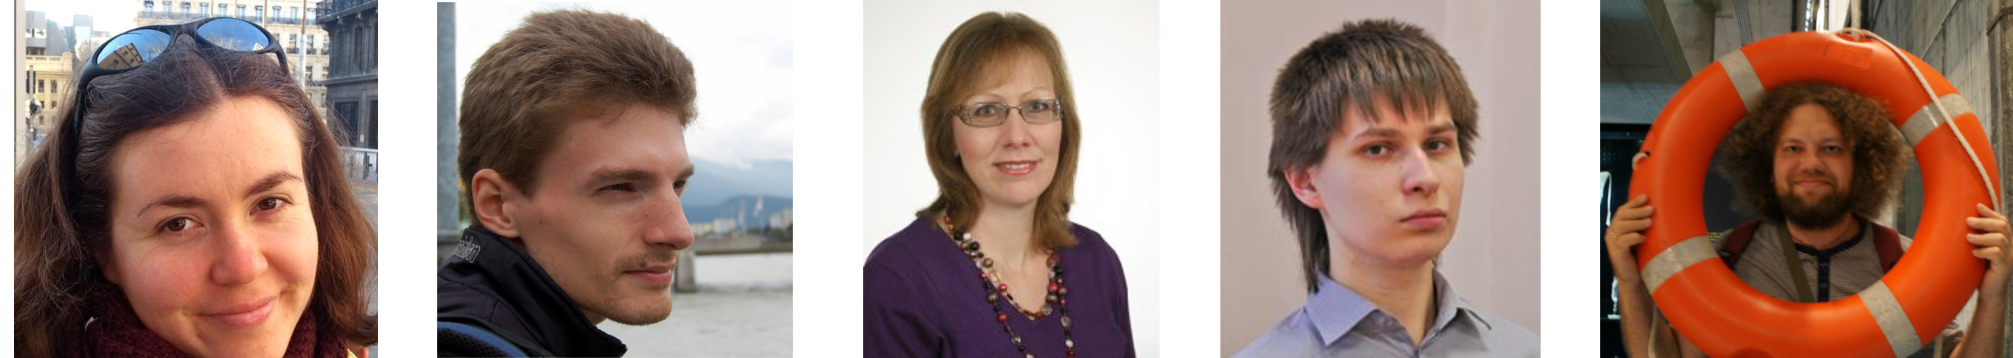
\includegraphics[width=0.99\textwidth]{figures/russe-team}
%%  \end{center}
%\end{frame}



\begin{frame}{A lexical sample WSI task}
  
  \begin{itemize}
  	\item \textbf{Target word}, e.g. ``bank''.
  	
  	\pause 
  	
  	\item \textbf{Contexts} where the word occurs, e.g.: 
  	\begin{itemize}
  	\item ``river \textbf{bank} is a slope beside a body of water''
  	\item ``\textbf{bank} is a financial institution that accepts deposits''
  	\item ``Oh, the \textbf{bank} was robbed. They took about a million dollars.''
  	\item ``\textbf{bank} of Elbe is a good and popular hangout spot complete with good food and fun''
  	\end{itemize}
  	
  	\pause 
  	
  	\item You need to \textbf{{group} the contexts by senses}:
  	\begin{itemize}
  	\item \textcolor{Cerulean}{``river \textbf{bank} is a slope beside a body of water''}
  	\item \textcolor{Cerulean}{``\textbf{bank} of Elbe is a good and popular hangout spot complete with good food and fun''}
  	\item \alert{``\textbf{bank} is a financial institution that accepts deposits''}
  	\item \alert{``Oh, the \textbf{bank} was robbed. They took about a million dollars.''}
  	\end{itemize}
  	 
  \end{itemize}
  
\end{frame}
%
%
%\begin{frame}{Dataset based on Wikipedia}
%
%{\centering
%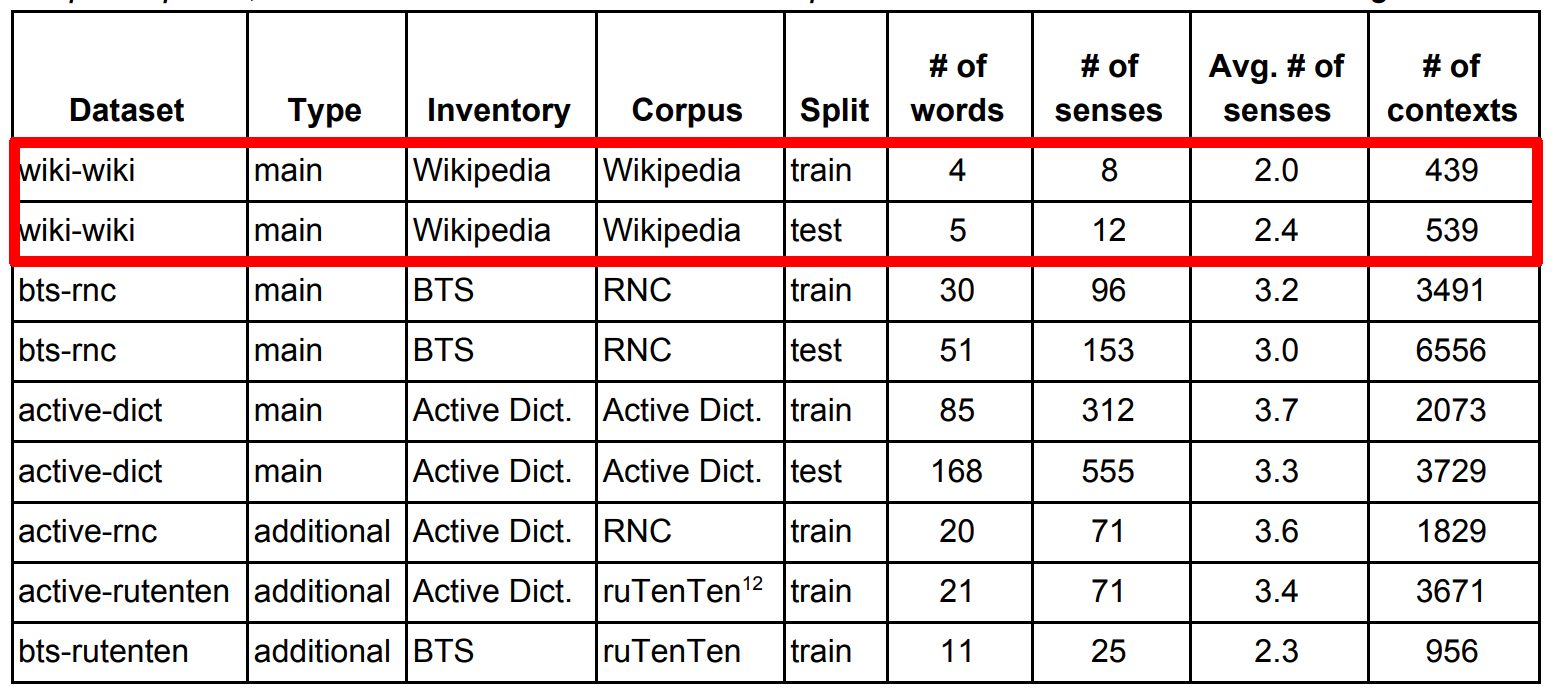
\includegraphics[width=1.0\textwidth]{figures/datasets1}
%}	
%\end{frame}
%
%
%\begin{frame}{Dataset based on RNC}
%
%{\centering
%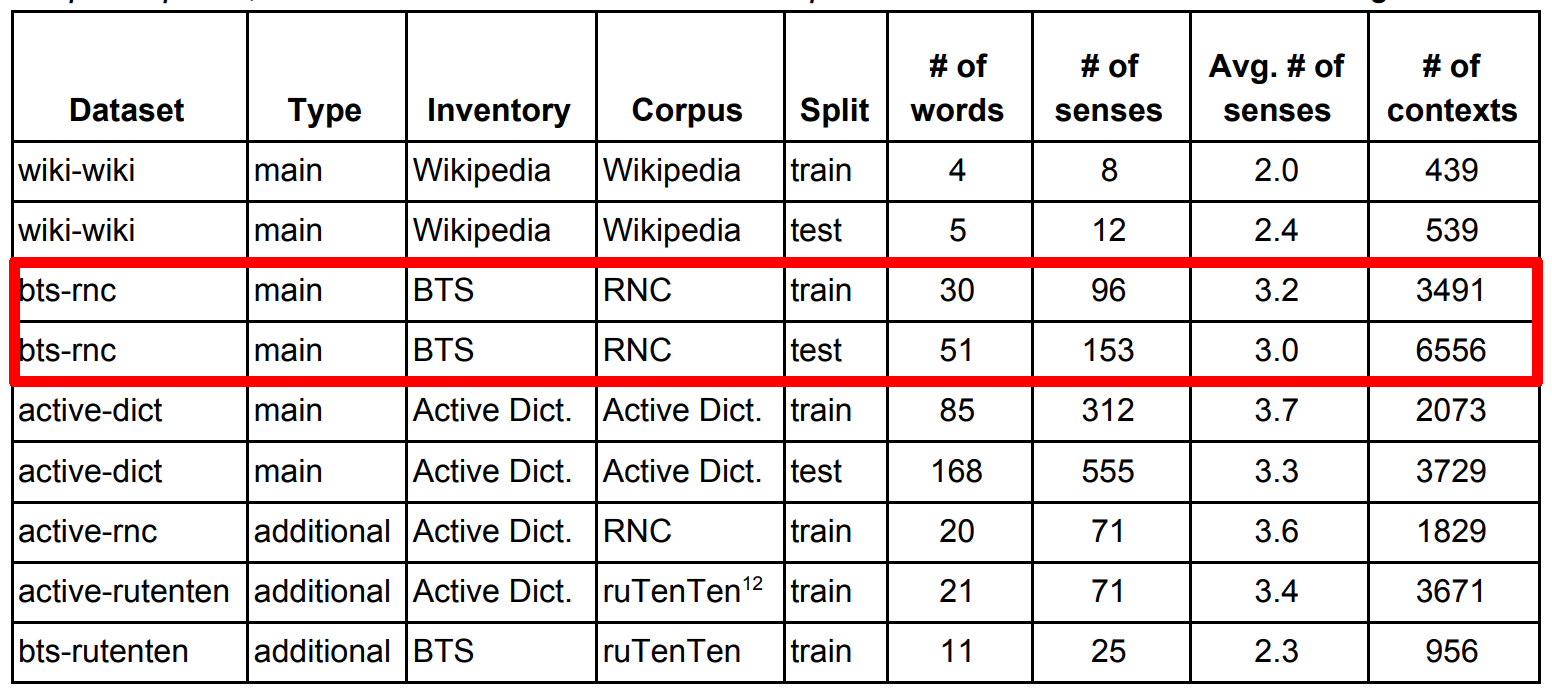
\includegraphics[width=1.0\textwidth]{figures/datasets2}
%}	
%\end{frame}
%
%
%\begin{frame}{Dataset based on dictionary glosses}
%
%{\centering
%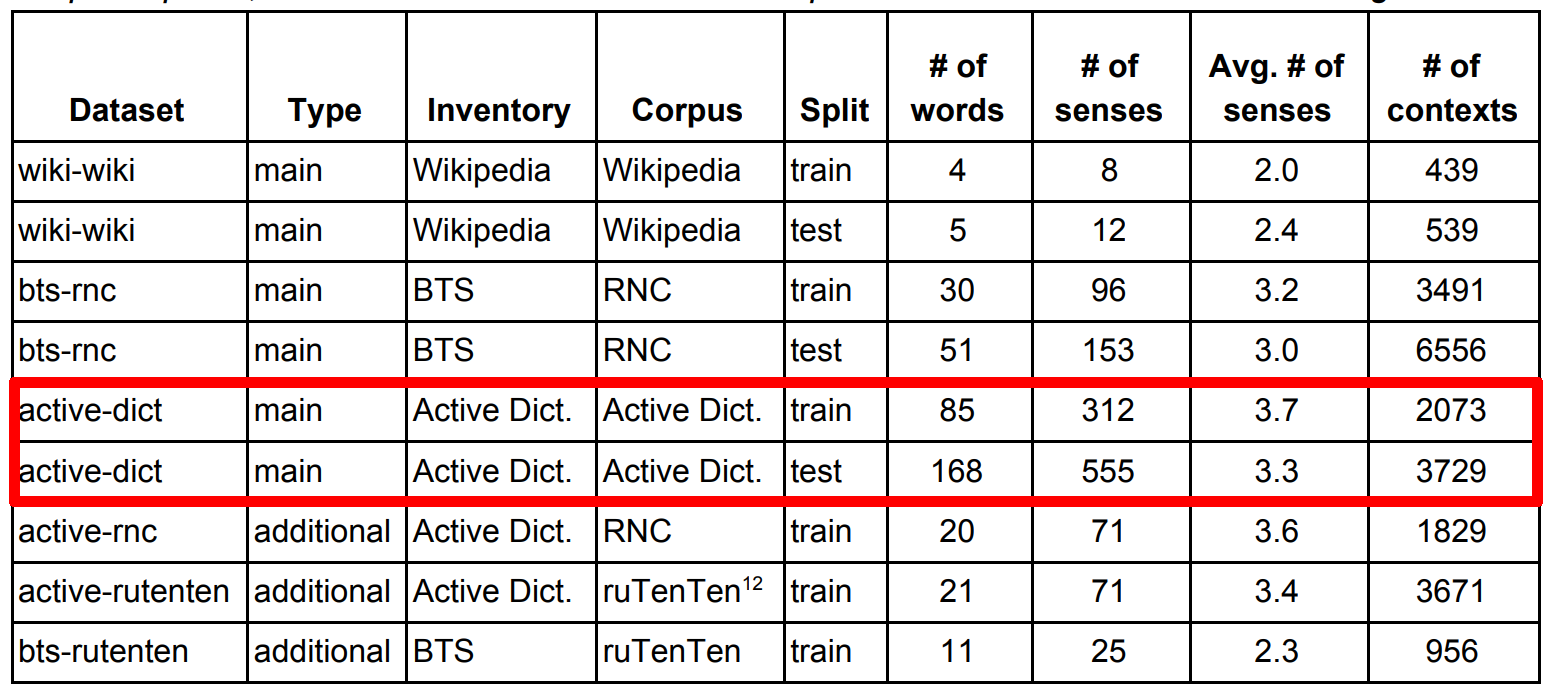
\includegraphics[width=1.0\textwidth]{figures/datasets3}
%}	
%\end{frame}
%
%
%
%\begin{frame}{A sample from the \textit{wiki-wiki} dataset }
%
%{\centering
%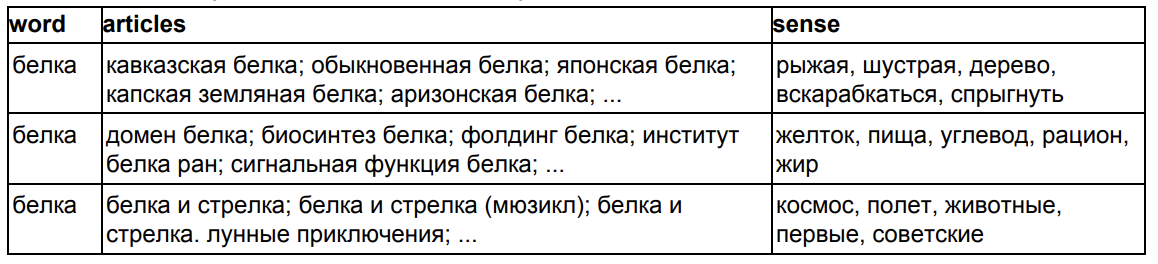
\includegraphics[width=1.0\textwidth]{figures/belka}
%}	
%\end{frame}
%
%
%
%\begin{frame}{A sample from the \textit{wiki-wiki} dataset }
%
%{\centering
%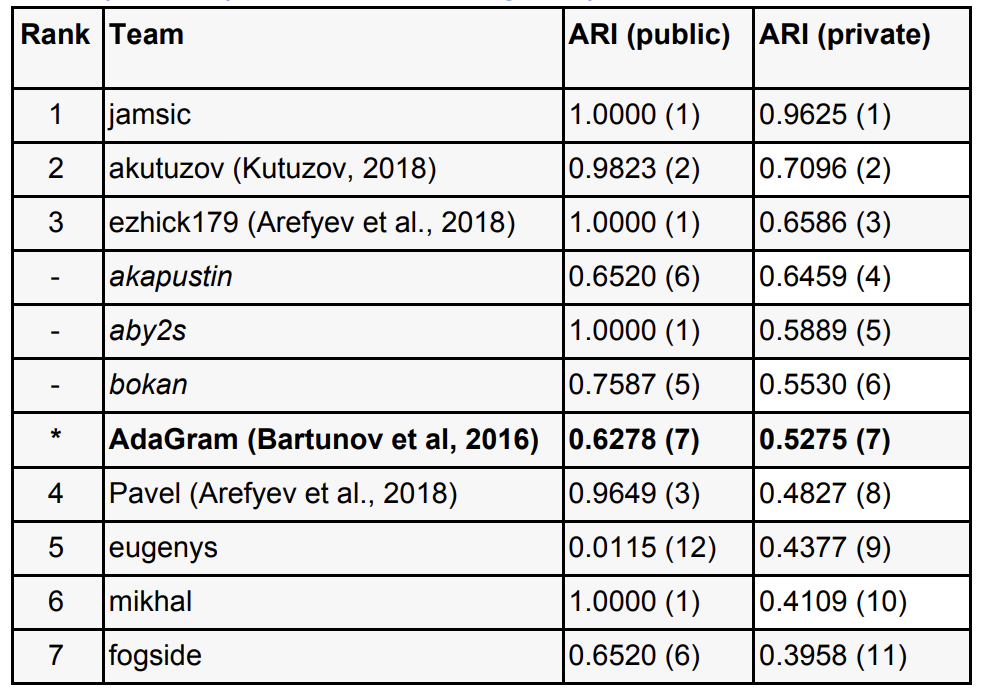
\includegraphics[width=.8\textwidth]{figures/wiki-wiki}
%}	
%\end{frame}
%
%
%
%\begin{frame}{A sample from the \textit{wiki-wiki} dataset }
%
%{\centering
%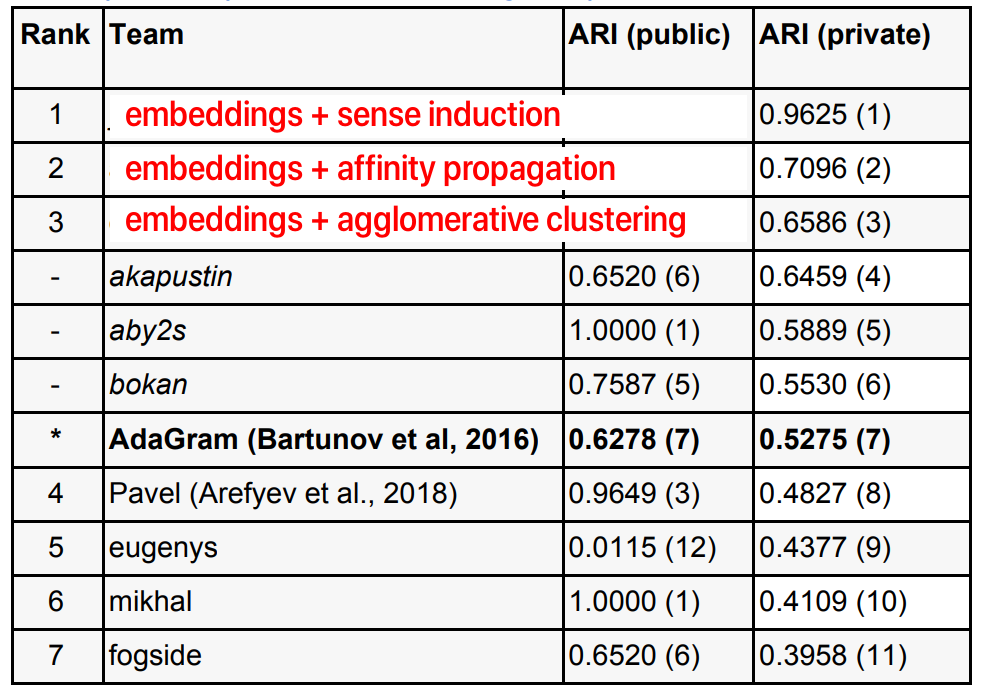
\includegraphics[width=.8\textwidth]{figures/wiki-wiki-top}
%}	
%\end{frame}
%
%
%
%\begin{frame}{A sample from the \textit{bts-rnc} dataset }
%
%{\centering
%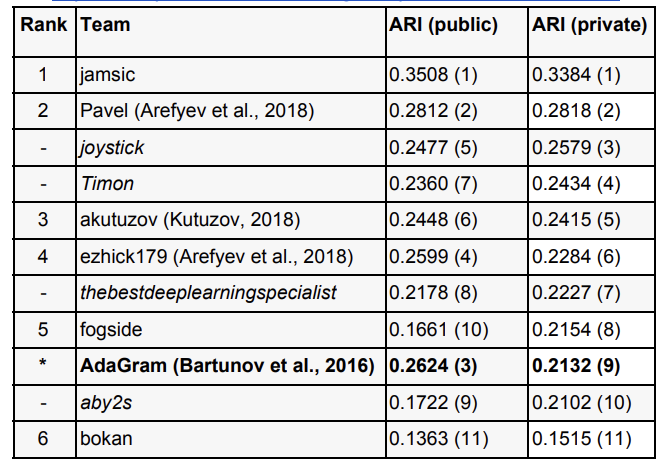
\includegraphics[width=.8\textwidth]{figures/bts}
%}	
%\end{frame}
%
%
%
%\begin{frame}{A sample from the \textit{active-dict} dataset }
%
%{\centering
%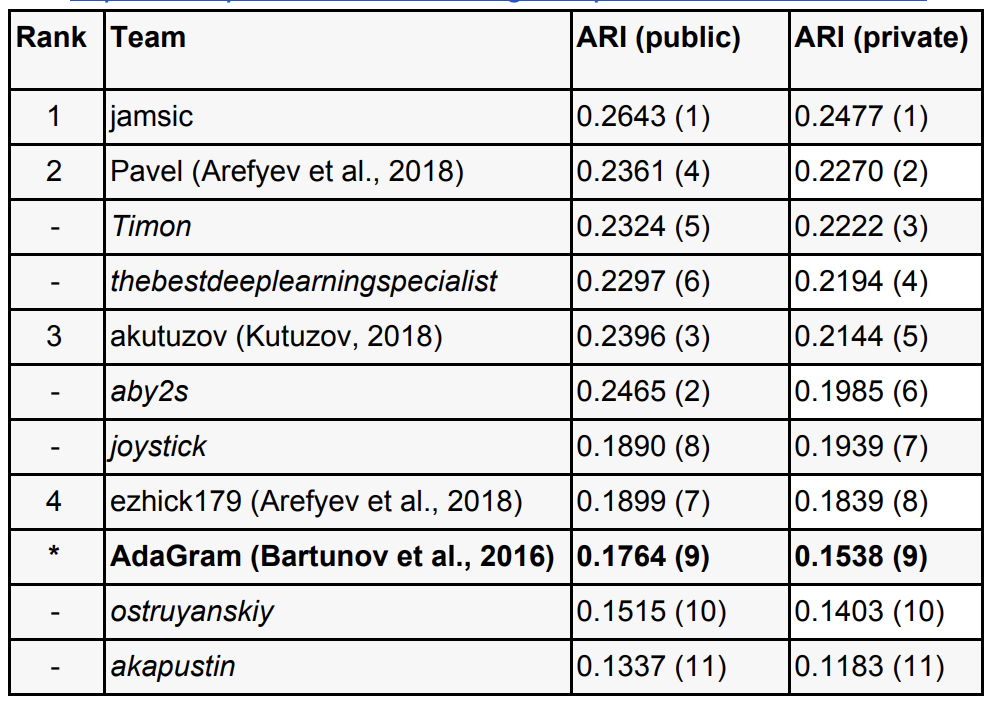
\includegraphics[width=.8\textwidth]{figures/active}
%}	
%\end{frame}



\begin{frame}{ Sense induction using clustering }


 \begin{center}
  	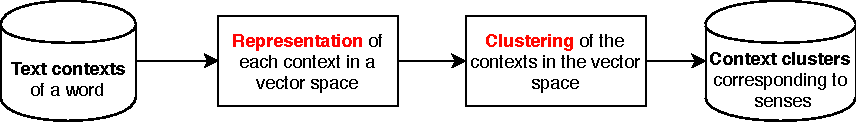
\includegraphics[width=0.99\textwidth]{figures/Clustering}
  \end{center}
  
  \pause 
  \begin{itemize}
  \item \textbf{\alert{Representation}}
  \begin{itemize}
  
  \item Sparse vector model (TF-IDF, etc.)
  \item Weighted (TF-IDF, $\chi^2$, etc.) sum of word embeddings
  \item Sentence embeddings (InterSent, Skip-Thougts, doc2vec, etc.)
  \end{itemize}
  
  \pause 
  \item \textbf{\alert{Clustering}}
  
  \begin{itemize}
  \item Affinity Propagation
  \item Agglomerative Clustering
  \item $k$-means
  \end{itemize} 	
  \end{itemize}


\end{frame}



\begin{frame}{ Sense induction using neighbors }

\begin{enumerate}
	\item \textbf{Get the neighbors} of a target word, e.g. \textbf{``bank''}:
	\begin{enumerate}
	\item \alert{lender}
	\item \textcolor{Cerulean}{river}
	\item \alert{citybank}
	\item \textcolor{Cerulean}{slope}
	\item ...
	\end{enumerate}
	
	\item Get \textbf{similar to ``bank''} and \textbf{dissimilar to \alert{``lender''}}:
	
	\begin{enumerate}
	\item \textcolor{Cerulean}{river}
	\item \textcolor{Cerulean}{slope}
	\item \textcolor{Cerulean}{land}
	\item ...
	\end{enumerate}
	 
\item \textbf{Compute distances} to \alert{\textbf{``lender''}} and \textcolor{Cerulean}{\textbf{``river''}}.
\end{enumerate}

\end{frame}





\begin{frame}{ Graph-vector sense induction }

\begin{enumerate}
\item \textbf{For} $i$-th neighbor of the target word $w$ among $k$ neigbours:

\begin{enumerate}
	\item Get a pair of opposite words for the $i$ neighbor: $(w_j, w_k)$
	\item Add them as as nodes: $V = V \cup \{w_j, w_k\}$
	\item Remember the pair as an anti-edge: $A = A \cup (w_j, w_k)$
\end{enumerate}

\pause 

\item \textbf{Build an ego network} $G = (V, E)$ of the word $w$:
\begin{enumerate}

\item $E$ are computed based on word similarities;
\item $E$ are pruned based on the anti-edge constraints: $E = E \smallsetminus
 A$.
	
\end{enumerate}

\pause 

\item \textbf{Cluster} the ego network of the word $w$.

\pause 

\item \textbf{Find cluster labels} by finding the central nodes in a cluster.

\end{enumerate}

\end{frame}






\begin{frame}{ Graph-vector sense induction }

\begin{itemize}
	\item \textbf{Get the neighbors} of a target word, e.g. \textbf{``java''}:
	\begin{enumerate}
	\item \alert{Python}
	\item \textcolor{Cerulean}{Borneo}
	\item \alert{C++}
	\item \textcolor{Cerulean}{Sumatra}
	\item \textcolor{Green}{Arabica}
    \item \textcolor{Green}{Robusta}
	\item \alert{Ruby}
	\item \alert{JavaScript}
	\item \textcolor{Cerulean}{Bali}

	\item ...
	\end{enumerate}

\end{itemize}

\end{frame}




\begin{frame}{ Graph-vector sense induction }

\begin{itemize}
	\item \textbf{Get the neighbors} of a target word, e.g. \textbf{``java''}:
	\begin{enumerate}
	\item \alert{Python} $\neq$ \textcolor{Cerulean}{Borneo}
	\item \textcolor{Cerulean}{Borneo} $\neq$ \alert{Scala}
	\item \alert{C++} $\neq$ \textcolor{Cerulean}{Borneo}
	\item \textcolor{Cerulean}{Sumatra} $\neq$ highway
	\item \textcolor{Green}{Arabica} $\neq$ \alert{Python}
    \item \textcolor{Green}{Robusta} $\neq$ \alert{Python}
	\item \alert{Ruby} $\neq$ \textcolor{Green}{Arabica}
	\item \textcolor{Cerulean}{Bali} $\neq$ North
	\end{enumerate}

\end{itemize}
\end{frame}




\begin{frame}{ Graph-vector sense induction }
\begin{itemize}

\item \textbf{Nodes}:

	\begin{enumerate}
	\item \alert{Python}
	\item \textcolor{Cerulean}{Borneo}
	\item \alert{C++}
	\item \textcolor{Green}{Arabica}
    \item \textcolor{Green}{Robusta}
	\item \alert{Ruby}
\end{enumerate}

\end{itemize}
\end{frame}





\begin{frame}{ Sense induction }


 \begin{center}
  	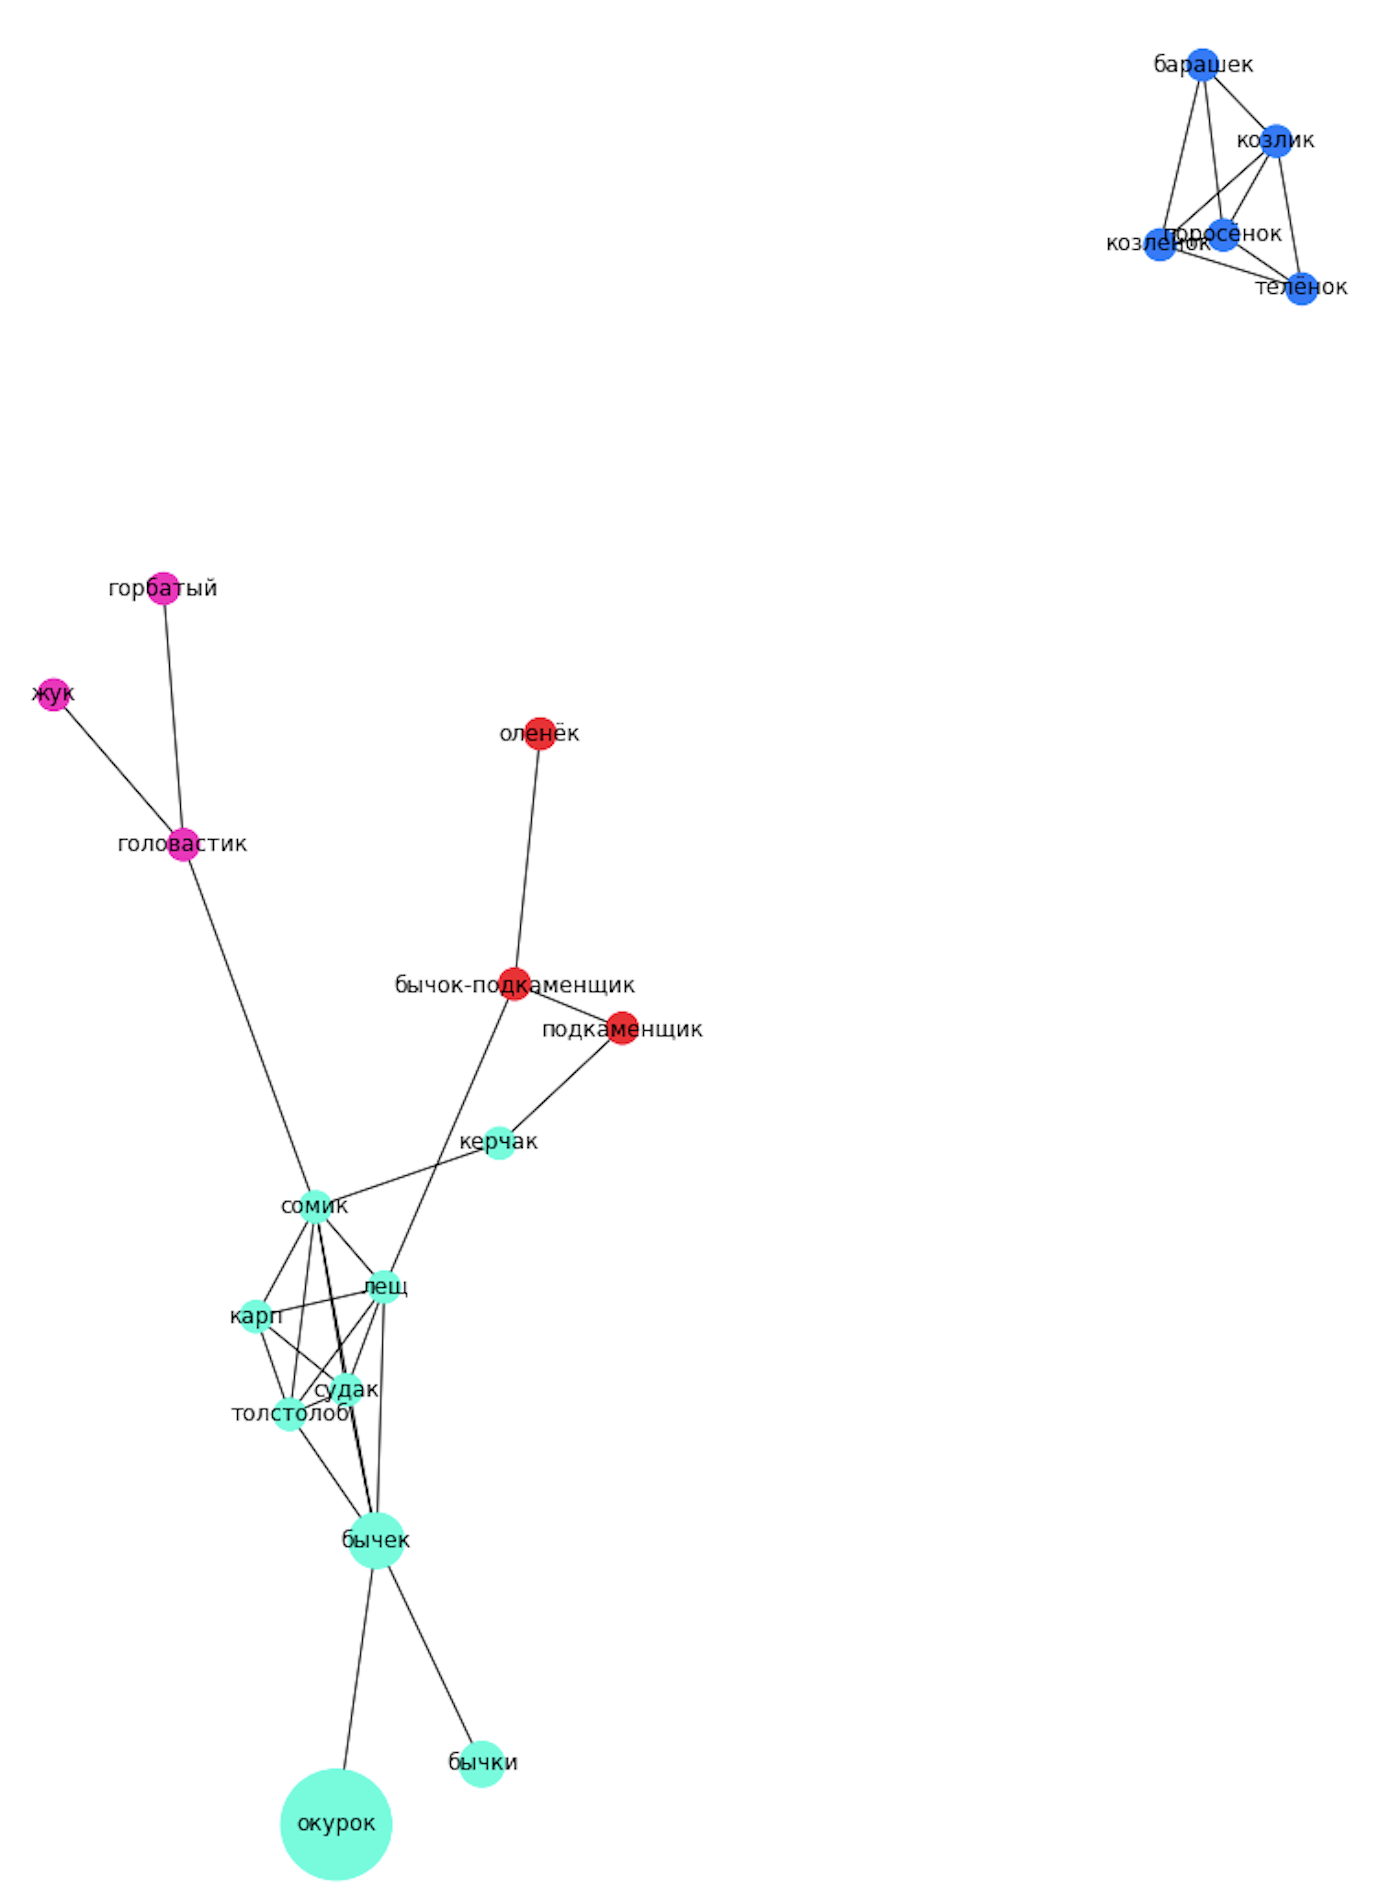
\includegraphics[height=0.69\textheight]{figures/bychok}
  \end{center}
  


\end{frame}




\begin{frame}{ Datasets }
\vspace{-10pt}

\begin{enumerate}
	\item SemEval 2007 
	\item SemEval 2010
	\item RUSSE 2018
	\item \textbf{SemEval 2019 Task 2 Subtask 1}:  
	\begin{itemize}
		\item Clustering of verb occurrences
		\item Assign occurrences of the target verbs to a number of clusters, in such a way that verbs belonging to the same cluster evoke the same frame type.
		\item gold annotations for this subtask are based on FrameNet
	\end{itemize}
	
\end{enumerate}

\pause 
\vspace{5pt}

\begin{itemize}
\footnotesize
\item Trump \textbf{leads} the world, backward.
\item Disrespecting international laws \textbf{leads} to many complications.
\item Rosenzweig \textbf{heads} the climate impacts section at NASA's Goddard Institute.
\end{itemize}

\end{frame}



\begin{frame}{ Datasets }
\vspace{-10pt}

\begin{enumerate}
	\item SemEval 2007 
	\item SemEval 2010
	\item RUSSE 2018
	\item \textbf{SemEval 2019 Task 2 Subtask 1}:  
	\begin{itemize}
		\item Clustering of verb occurrences
		\item Assign occurrences of the target verbs to a number of clusters, in such a way that verbs belonging to the same cluster evoke the same frame type.
		\item gold annotations for this subtask are based on FrameNet
	\end{itemize}
	
\end{enumerate}


\vspace{5pt}

\begin{itemize}
\footnotesize
\item \alert{Trump \textbf{leads} the world, backward.}
\item \textcolor{Cerulean}{Disrespecting international laws \textbf{leads} to many complications.}
\item \alert{Rosenzweig \textbf{heads} the climate impacts section at NASA's Goddard Institute.}
\end{itemize}

\end{frame}


